% Beamer version of the "Sorting Networks of Logarithmic Depth" slide deck.
% Mirrors the HTML deck in slides/project (same order, palette and diagrams).
% Diagrams are drawn in TikZ using the HTML deck's pixel coordinates (1920 x 1080 canvas = 16cm x 9cm).
% Compile with: latexmk -pdf slides_beamer.tex
% Speaker notes are included with \note{}; to show them, add \setbeameroption{show notes on second screen=right}.
\documentclass[aspectratio=169,9pt,xcolor=table]{beamer}

\usepackage[T1]{fontenc}
\usepackage[sfdefault]{plex-sans}
\usepackage[lining]{ebgaramond}
\usefonttheme[onlymath]{serif}
\usepackage{amsmath,amssymb}
\usepackage{booktabs}
\usepackage{tikz}
\usetikzlibrary{shapes.arrows,arrows.meta}
\usepackage[most]{tcolorbox}

% ---------- palette ----------
\definecolor{navy}{HTML}{14213D}
\definecolor{ink}{HTML}{3A4659}
\definecolor{paper}{HTML}{F7F5EF}
\definecolor{paperalt}{HTML}{ECE8DD}
\definecolor{rust}{HTML}{A63D26}
\definecolor{rustlight}{HTML}{E9A58F}
\definecolor{steel}{HTML}{2F5F8A}
\definecolor{mist}{HTML}{C9D3E0}
\definecolor{muted}{HTML}{5F6B7D}
\definecolor{hl}{HTML}{FBE9E3}
\definecolor{softrust}{HTML}{F2D9D2}
\definecolor{amber}{HTML}{B7791F}
\definecolor{caveatbg}{HTML}{FFF6E5}
\definecolor{caveatfg}{HTML}{4A3B1C}
\definecolor{wire}{HTML}{9AA6B8}

% ---------- beamer theme ----------
\setbeamertemplate{navigation symbols}{}
\setbeamersize{text margin left=1.07cm, text margin right=1.07cm}
\setbeamercolor{background canvas}{bg=paper}
\setbeamercolor{normal text}{fg=ink}
\setbeamercolor{frametitle}{fg=navy}
\setbeamercolor{framesubtitle}{fg=rust}
\setbeamercolor{structure}{fg=steel}
\setbeamerfont{frametitle}{family=\rmfamily, series=\bfseries, size=\huge}
\setbeamerfont{framesubtitle}{family=\sffamily, size=\tiny, series=\bfseries}
\setbeamertemplate{itemize item}{\color{steel}\raisebox{0.15ex}{\scriptsize$\bullet$}}
\setbeamertemplate{enumerate item}{\color{rust}\bfseries\insertenumlabel.}

\setbeamertemplate{frametitle}{%
  \vspace*{0.55cm}%
  {\usebeamercolor[fg]{framesubtitle}\usebeamerfont{framesubtitle}\MakeUppercase{\insertframesubtitle}\par}%
  \vspace{0.12cm}%
  {\usebeamercolor[fg]{frametitle}\usebeamerfont{frametitle}\insertframetitle\par}%
  \vspace{0.1cm}%
}
\setbeamertemplate{footline}{%
  \hspace*{1.07cm}{\color{muted}\fontsize{5}{6}\selectfont Sorting networks of logarithmic depth\hfill\insertframenumber}\hspace*{1.07cm}%
  \vspace*{0.45cm}%
}

% Background variants: use inside a group around a frame.
\newcommand{\altstyle}{\setbeamercolor{background canvas}{bg=paperalt}}
\newcommand{\darkstyle}{%
  \setbeamercolor{background canvas}{bg=navy}%
  \setbeamercolor{normal text}{fg=mist}%
  \setbeamercolor{frametitle}{fg=paper}%
  \setbeamercolor{framesubtitle}{fg=rustlight}%
}

% ---------- building blocks ----------
\newlength{\px}\setlength{\px}{0.0083333cm} % one pixel of the 1920px-wide HTML canvas
\tikzset{pxgrid/.style={x=\px, y=-\px}}
% comparator at x between wires y1 and y2 (current colour)
\newcommand{\cmp}[4][10]{\draw[line width=6\px] (#2,#3) -- (#2,#4); \fill (#2,#3) circle[radius=#1\px]; \fill (#2,#4) circle[radius=#1\px];}

\newtcolorbox{card}[2][steel]{enhanced, colback=white, colframe=white, boxrule=0pt, arc=1mm,
  borderline north={2pt}{0pt}{#1}, left=6pt, right=6pt, top=6pt, bottom=6pt,
  drop shadow={opacity=0.08}, before upper={\raggedright{\color{#1}\fontsize{6}{7}\selectfont\bfseries #2\par}\vspace{3pt}}}
\newtcolorbox{caveat}{enhanced, colback=caveatbg, colframe=caveatbg, boxrule=0pt, sharp corners,
  borderline west={2pt}{0pt}{amber}, left=6pt, right=6pt, top=4pt, bottom=4pt, fontupper=\footnotesize\raggedright\color{caveatfg}}
\newtcolorbox{statement}{enhanced, colback=white, colframe=white, boxrule=0pt, sharp corners,
  borderline west={3pt}{0pt}{rust}, left=10pt, right=10pt, top=8pt, bottom=8pt}
\newtcolorbox{step}[1]{enhanced, colback=white, colframe=white, boxrule=0pt, arc=1mm, left=6pt, right=6pt, top=6pt, bottom=6pt,
  before upper={{\rmfamily\bfseries\Huge\color{rust}#1\par}\vspace{2pt}}, fontupper=\small\raggedright}
\newcommand{\rarrow}{\tikz\node[single arrow, fill=rust, minimum height=0.55cm, single arrow head extend=2pt, inner sep=1.5pt]{};}
\renewcommand{\arraystretch}{1.35}
\newcommand{\bigmath}[1]{{\rmfamily\bfseries\color{navy}#1}}

\title{Sorting Networks of Logarithmic Depth}

\begin{document}

% ======================= 1. Cover =======================
\begingroup\darkstyle
\begin{frame}[plain]
\begin{tikzpicture}[remember picture, overlay, pxgrid, shift={(current page.north west)}]
  \begin{scope}[shift={(1152,260)}, opacity=0.35]
    \foreach \y in {20,94,168,242,316,390,464,538} \draw[mist, line width=3\px] (0,\y) -- (640,\y);
    \begin{scope}[rustlight]
      \cmp[9]{70}{20}{94} \cmp[9]{70}{168}{242} \cmp[9]{70}{316}{390} \cmp[9]{70}{464}{538}
      \cmp[9]{180}{20}{168} \cmp[9]{200}{94}{242} \cmp[9]{180}{316}{464} \cmp[9]{200}{390}{538}
      \cmp[9]{300}{94}{168} \cmp[9]{300}{390}{464}
      \cmp[9]{410}{20}{316} \cmp[9]{430}{94}{390} \cmp[9]{450}{168}{464} \cmp[9]{470}{242}{538}
      \cmp[9]{570}{168}{316} \cmp[9]{590}{242}{390}
    \end{scope}
  \end{scope}
\end{tikzpicture}%
\vspace*{1.2cm}
\begin{minipage}{7.4cm}\raggedright
{\color{rustlight}\fontsize{6}{7}\selectfont\bfseries RESEARCH REPORT \textperiodcentered\ AN EXCELLENT SORT\par}
\vspace{0.3cm}
{\rmfamily\bfseries\fontsize{26}{29}\selectfont\color{paper}Sorting Networks of Logarithmic Depth\par}
\vspace{0.35cm}
{\large\color{mist}What AI agents found about lower bounds, explicit constructions and the AKS network\par}
\end{minipage}
\note{This talk summarizes a project that used AI agents (Claude, ChatGPT and the Open Math model) to study sorting networks: how shallow they can be, how to build shallow ones, and how to understand the famous AKS construction better. I will cover what sorting networks are, what the project set out to do, the three main outcomes, and then what did not work.}
\end{frame}
\endgroup

% ======================= 2. Sequential sorting =======================
\begingroup\altstyle
\begin{frame}{One comparison at a time, sorting is solved}{Background \textperiodcentered\ Sequential sorting}
\begin{columns}[c]
\begin{column}{0.42\textwidth}
\bigmath{\fontsize{40}{44}\selectfont $\Theta(n\log n)$}\par\vspace{0.2cm}
comparisons are necessary and sufficient to sort $n$ items.
\end{column}
\begin{column}{0.54\textwidth}
\begin{card}{Lower bound}
Each comparison has two outcomes, and there are $n!$ orderings to tell apart. So at least $\log_2 n! \approx n\log_2 n$ comparisons are needed.
\end{card}
\begin{card}{Matching algorithms}
Mergesort and heapsort achieve $O(n\log n)$ in the worst case, and quicksort on average.
\end{card}
\end{column}
\end{columns}
\vspace{0.4cm}
{\color{navy}The open questions start when comparisons can be made \textbf{in parallel}.}
\note{Before parallel sorting, recall the sequential story. In the comparison model, an algorithm learns about the input only by comparing pairs. There are n factorial possible orderings and each comparison halves the possibilities at best, so we need about n log n comparisons. Mergesort and heapsort match this in the worst case, quicksort on average. So sequential comparison sorting is essentially solved. If comparisons can run in parallel, the question becomes how many rounds are needed. Since at most n/2 disjoint comparisons fit in one round, at least about 2 log n rounds are needed.}
\end{frame}
\endgroup

% ======================= 3. Sorting networks =======================
\begin{frame}{A sorting network is a fixed circuit of comparisons}{Background}
\begin{columns}[c]
\begin{column}{0.48\textwidth}
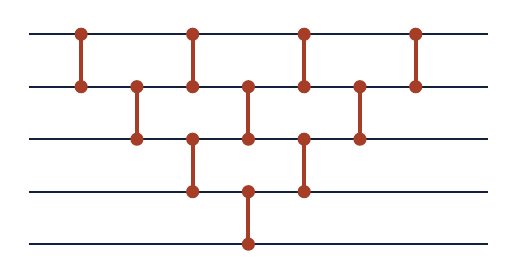
\begin{tikzpicture}[pxgrid]
  \foreach \y in {50,130,210,290,370} \draw[navy, line width=3\px] (30,\y) -- (730,\y);
  \begin{scope}[rust]
    \cmp{110}{50}{130} \cmp{195}{130}{210} \cmp{280}{210}{290} \cmp{280}{50}{130}
    \cmp{365}{290}{370} \cmp{365}{130}{210} \cmp{450}{210}{290} \cmp{450}{50}{130}
    \cmp{535}{130}{210} \cmp{620}{50}{130}
  \end{scope}
\end{tikzpicture}\par\vspace{0.15cm}
{\scriptsize\color{muted}Bubble sort on 5 wires: 10 comparators, but only 7 parallel layers ($2n-3$).}
\end{column}
\begin{column}{0.48\textwidth}
\textbf{Wires} carry items left to right.\par\medskip
\textbf{Comparators} put the smaller item on the upper wire and the larger on the lower one.\par\medskip
\textbf{Layers} are comparators on disjoint wires, run at the same time.\par\medskip
\textbf{Depth} is the number of layers. $D(n)$ is the least depth that sorts every input of size $n$.
\end{column}
\end{columns}
\note{A sorting network is an oblivious algorithm: the comparisons are fixed in advance and do not depend on the data. That makes it suitable for hardware and parallel machines. The cost we care about is depth, the number of parallel rounds. Bubble sort uses n choose 2 comparisons, but they can be packed into 2n - 3 layers. A useful tool throughout is the zero-one principle: a network sorts all inputs if it sorts all inputs made of 0s and 1s.}
\end{frame}

% ======================= 4. Batcher =======================
\begingroup\altstyle
\begin{frame}{Divide and conquer with an exact halving step}{Background \textperiodcentered\ Batcher's sort}
\begin{columns}[c]
\begin{column}{0.46\textwidth}
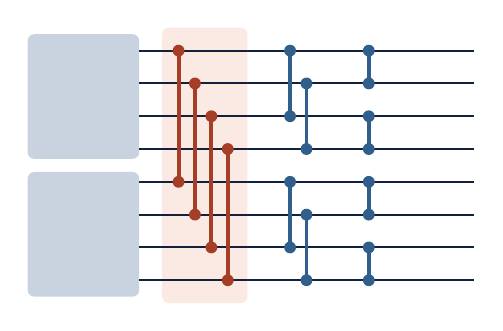
\begin{tikzpicture}[pxgrid]
  \fill[mist, rounded corners=10\px] (20,20) rectangle (190,210);
  \fill[mist, rounded corners=10\px] (20,230) rectangle (190,420);
  \fill[hl, rounded corners=10\px] (225,10) rectangle (355,430);
  \foreach \y in {45,95,145,195,245,295,345,395} \draw[navy, line width=3\px] (190,\y) -- (700,\y);
  \begin{scope}[rust]
    \cmp[9]{250}{45}{245} \cmp[9]{275}{95}{295} \cmp[9]{300}{145}{345} \cmp[9]{325}{195}{395}
  \end{scope}
  \begin{scope}[steel]
    \cmp[9]{420}{45}{145} \cmp[9]{445}{95}{195} \cmp[9]{420}{245}{345} \cmp[9]{445}{295}{395}
    \cmp[9]{540}{45}{95} \cmp[9]{540}{145}{195} \cmp[9]{540}{245}{295} \cmp[9]{540}{345}{395}
  \end{scope}
\end{tikzpicture}\par\vspace{0.1cm}
{\scriptsize\textcolor{steel}{\textbf{Grey:} sort halves}\quad \textcolor{rust}{\textbf{Red:} halving layer}\quad \textcolor{muted}{\textbf{Blue:} recurse}}
\end{column}
\begin{column}{0.50\textwidth}
\textbf{1.} Sort the two halves in parallel, one ascending and one descending.\par\medskip
\textbf{2.} One layer comparing wire $i$ with wire $i+n/2$ now \textbf{exactly halves} the items: every item on top is smaller than every item below.\par\medskip
\textbf{3.} Recurse on each half. Merging costs $\log_2 n$ layers, so sorting costs $\tfrac12\log_2 n\,(\log_2 n+1)$.
\end{column}
\end{columns}
\note{This is Batcher's bitonic sort, viewed as halving plus divide and conquer. After the two halves are sorted in opposite directions, the sequence is bitonic, and a single layer of comparators between wire i and wire i + n/2 splits it exactly: the n/2 smallest items end up on top. Each half is again bitonic, so we recurse. The halving step is only one layer, but it is exact only because we first paid to sort both halves. That recursive sorting is what costs log squared depth. An exact halver on arbitrary inputs provably needs depth at least log2 n.}
\end{frame}
\endgroup

% ======================= 5. epsilon-halver =======================
\begin{frame}{AKS halves cheaply and corrects the errors}{Background \textperiodcentered\ The AKS idea}
\begin{columns}[c]
\begin{column}{0.42\textwidth}
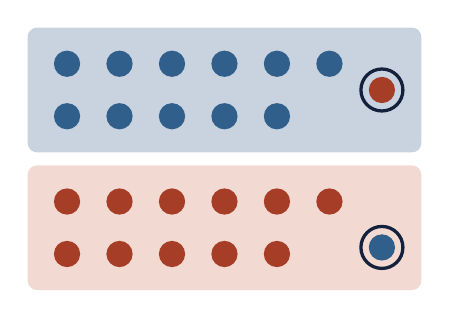
\begin{tikzpicture}[pxgrid]
  \fill[mist, rounded corners=14\px] (20,20) rectangle (620,210);
  \fill[softrust, rounded corners=14\px] (20,230) rectangle (620,420);
  \foreach \x in {80,160,240,320,400,480} {\fill[steel] (\x,75) circle[radius=20\px]; \fill[rust] (\x,285) circle[radius=20\px];}
  \foreach \x in {80,160,240,320,400} {\fill[steel] (\x,155) circle[radius=20\px]; \fill[rust] (\x,365) circle[radius=20\px];}
  \fill[steel] (560,355) circle[radius=20\px]; \fill[rust] (560,115) circle[radius=20\px];
  \draw[navy, line width=5\px] (560,115) circle[radius=32\px] (560,355) circle[radius=32\px];
\end{tikzpicture}\par\vspace{0.1cm}
{\scriptsize\textcolor{steel}{\textbf{Blue:} small items}\quad \textcolor{rust}{\textbf{Red:} large items}\quad \textcolor{muted}{\textbf{Circled:} misplaced}}
\end{column}
\begin{column}{0.54\textwidth}
\textbf{$\varepsilon$-halver:} of the $k$ smallest items, at most $\varepsilon k$ end up in the bottom half (and likewise for the largest).\par\medskip
\textbf{Constant depth:} built from a few matchings of an expander graph, independent of $n$.\par\medskip
\textbf{The catch:} halving and recursing lets errors pile up. AKS keeps a tree of bags and sends items that look out of place \textbf{back up} to be re-sorted.
\end{column}
\end{columns}
\note{If we could halve exactly in constant depth, halve-then-recurse would sort in O(log n) depth. But an exact halver needs depth at least log2 n. AKS gives up exactness: an epsilon-halver of constant depth misplaces a small fraction of items. Such halvers come from expander graphs: each layer is a matching, and a constant number of matchings suffice for any fixed epsilon. The difficulty is that misplaced items would end up in the wrong subtree forever. The AKS tree of bags fixes this: at every stage each bag sends its most extreme items up to its parent, so a misplaced item gets a chance to move to the correct branch.}
\end{frame}

% ======================= 6. Expander =======================
\begingroup\altstyle
\begin{frame}{A bipartite expander gives a constant-depth halver}{Background \textperiodcentered\ Building an $\varepsilon$-halver}
\begin{columns}[c]
\begin{column}{0.42\textwidth}
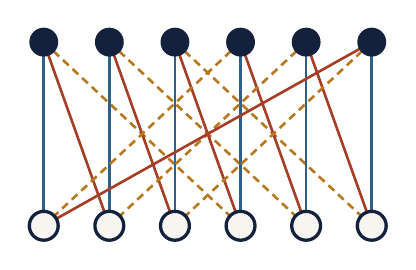
\begin{tikzpicture}[pxgrid]
  \foreach \i in {0,...,5} {
    \pgfmathtruncatemacro{\a}{mod(\i+1,6)} \pgfmathtruncatemacro{\b}{mod(\i+3,6)}
    \draw[steel, line width=4\px] (70+100*\i,80) -- (70+100*\i,360);
    \draw[rust, line width=4\px] (70+100*\i,80) -- (70+100*\a,360);
    \draw[amber, line width=4\px, dash pattern=on 12\px off 8\px] (70+100*\i,80) -- (70+100*\b,360);
  }
  \foreach \i in {0,...,5} {
    \fill[navy] (70+100*\i,80) circle[radius=22\px];
    \draw[navy, fill=paper, line width=5\px] (70+100*\i,360) circle[radius=22\px];
  }
\end{tikzpicture}\par\vspace{0.1cm}
{\scriptsize\textbf{Top row:} top-half wires\quad \textbf{Bottom row:} bottom-half wires\par}
{\tiny\color{muted}Each colour is one perfect matching, which is one layer of comparators (minimum to the top).\par}
\end{column}
\begin{column}{0.54\textwidth}
\textbf{1. Layers.} A $d$-regular bipartite graph between the halves splits into $d$ perfect matchings (Hall's theorem). Each becomes one layer.\par\medskip
\textbf{2. Stuck items.} A large item that ends on top was never displaced, so every wire it met holds a large item too.\par\medskip
\textbf{3. Expansion.} Any small set $S$ on top has at least $\frac{1-\varepsilon}{\varepsilon}|S|$ neighbours. With $k$ large items, the stuck set has $|S|\le\varepsilon k$.
\end{column}
\end{columns}
\note{Think in zero-one terms, with k ones (large items) and k at most n/2. Each layer compares a top wire with a bottom wire and puts the minimum on top. A top wire that ever holds a 0 keeps a 0 forever, and a bottom wire that ever holds a 1 keeps a 1. So if a top wire holds a 1 at the end, it held a 1 the whole time, and every bottom wire it was compared with received a 1 and kept it. So the stuck set S and its neighbourhood N(S) all hold ones: |S| + |N(S)| <= k. The expander guarantees |N(S)| >= ((1 - eps)/eps)|S| for every S of size at most eps n/2, so |S| + |N(S)| >= |S|/eps. If more than eps k ones were stuck, a subset of size about eps k would already have more than k ones around it, a contradiction. The degree d depends only on eps, not on n, so the depth is constant.}
\end{frame}
\endgroup

% ======================= 7. Landscape =======================
\begingroup\altstyle
\begin{frame}{Theory says $O(\log n)$; practice is stuck at $\log^2 n$}{Background}
\small
\rowcolors{2}{}{}
\begin{tabular}{p{0.40\textwidth}p{0.26\textwidth}p{0.24\textwidth}}
\toprule
\textbf{Result} & \textbf{Depth} & \textbf{Comment}\\
\midrule
Batcher (1968) & $\tfrac12\log n(\log n+1)$ & Simple, used in practice\\
\rowcolor{hl} Ajtai, Koml\'os, Szemer\'edi (1983) & $O(\log n)$ & Huge constant\\
Paterson (1990) & $\approx 6100\log n$ & Simplified AKS\\
Chv\'atal (1992) & $\approx 1830\log n$ & For $n\ge 2^{78}$\\
Lower bound (Kahale et al., 1995) & $3.27\log n$ & Best known\\
Exact values of $D(n)$ & known for $n\le 17$ & SAT solvers\\
\bottomrule
\end{tabular}\par\vspace{0.4cm}
{\color{navy}AKS only beats Batcher once $\log_2 n$ is in the thousands. There is a large gap between lower and upper bounds, for both small and large $n$.}
\note{The headline tension: AKS proved logarithmic depth is possible, but the constant is so large that Batcher's simple log-squared networks are better for any n we could ever use. Even with Chvatal's improved constant of about 1830, the crossover is around n = 2 to the 3600. On the lower-bound side we only know about 3.27 log n. And for concrete small n, exact optimal depths are known only up to 17 inputs.}
\end{frame}
\endgroup

% ======================= 8. Purpose =======================
\begin{frame}{Use AI agents to understand shallow sorting networks better}{Purpose of this effort}
\begin{columns}[t]
\begin{column}{0.48\textwidth}
\begin{card}{AKS analysis}A simpler, clearer account of why the AKS network works\end{card}
\begin{card}{Lower bounds}Explain why AKS needs its size, and give simpler proofs of known bounds\end{card}
\end{column}
\begin{column}{0.48\textwidth}
\begin{card}{New constructions}$O(\log n)$-depth networks that are simpler or connect to other mathematics\end{card}
\begin{card}{Fixed $n$}Find shallower sorting networks for specific values of $n$\end{card}
\end{column}
\end{columns}
\vspace{0.2cm}
{\scriptsize\color{muted}Agents used: the Open Math model, Claude and ChatGPT.}
\note{The project had four aims. The main one was to simplify the analysis of AKS. Alongside that we looked for new constructions, for lower bounds that would explain the structure of AKS, and for better networks at specific sizes. Several AI systems were used, and outcomes are attributed to the system that produced them.}
\end{frame}

% ======================= 9. Outcomes =======================
\begingroup\altstyle
\begin{frame}{Three concrete outcomes}{Statement of outcomes}
\begin{columns}[t]
\begin{column}{0.31\textwidth}
\begin{card}{Claude and ChatGPT}{\rmfamily\bfseries\large\color{navy}Lower bounds by hand\par}\smallskip
A short proof that $D(n)\ge D(\lceil n/2\rceil)+2$. It improves the lower bound for $D(32)$ from 10 to 11, with no SAT solver.\end{card}
\end{column}
\begin{column}{0.31\textwidth}
\begin{card}{Open Math model}{\rmfamily\bfseries\large\color{navy}AKS constants\par}\smallskip
Improved constants for AKS-style networks, and a correction to a constraint in Seiferas's analysis.\end{card}
\end{column}
\begin{column}{0.31\textwidth}
\begin{card}{Claude}{\rmfamily\bfseries\large\color{navy}Shallower networks\par}\smallskip
Verified networks on 128 and 1024 wires that are one layer shallower than previously known constructions.\end{card}
\end{column}
\end{columns}
\vspace{0.2cm}
{\color{muted}A potential-function view of AKS was also attempted, but did not give new insight.}
\note{These are the three outcomes listed in the report. The rest of the talk goes through each one, then covers the negative results. Note the attribution: each outcome is credited to the AI system that produced it.}
\end{frame}
\endgroup

% ======================= 10. Halving lemma statement =======================
\begingroup\darkstyle
\begin{frame}{The halving lemma}{Outcome 1 \textperiodcentered\ Lower bounds for small $n$}
\vspace{0.6cm}
{\color{paper}\fontsize{34}{38}\selectfont $D(n)\;\ge\; D(\lceil n/2\rceil)+2$\par}
\vspace{0.6cm}
{\Large\color{mist}Sorting $n$ items always takes at least two more layers than sorting half of them.\par}
\note{This holds for every n at least 3. Iterating it gives D(n) >= 2 ceil(log2 n) - 1. It is weaker than the asymptotic lower bounds, but for concrete n in the 20s to 60s, combined with the SAT-computed values up to 17, it gives new bounds.}
\end{frame}
\endgroup

% ======================= 11. Halving proof =======================
\begin{frame}{Freeze half the wires for two layers}{Outcome 1 \textperiodcentered\ Proof idea}
\begin{columns}[c]
\begin{column}{0.46\textwidth}
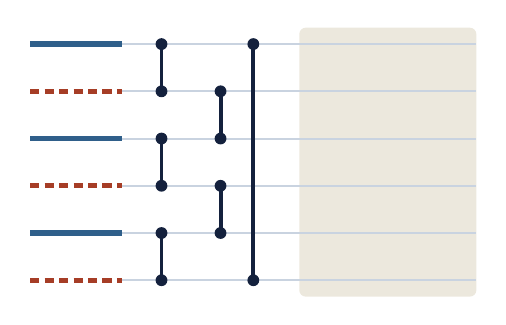
\begin{tikzpicture}[pxgrid]
  \fill[paperalt, rounded corners=10\px] (430,15) rectangle (700,425);
  \foreach \y in {40,112,184,256,328,400} \draw[mist, line width=3\px] (160,\y) -- (700,\y);
  \foreach \y in {40,184,328} \draw[steel, line width=8\px] (20,\y) -- (160,\y);
  \foreach \y in {112,256,400} \draw[rust, line width=8\px, dash pattern=on 14\px off 8\px] (20,\y) -- (160,\y);
  \begin{scope}[navy]
    \cmp[9]{220}{40}{112} \cmp[9]{220}{184}{256} \cmp[9]{220}{328}{400}
    \cmp[9]{310}{112}{184} \cmp[9]{310}{256}{328} \cmp[9]{360}{40}{400}
  \end{scope}
\end{tikzpicture}\par\vspace{0.1cm}
{\scriptsize\textcolor{steel}{\textbf{Solid:} variables}\quad \textcolor{rust}{\textbf{Dashed:} $\pm\infty$ constants}\quad \textcolor{muted}{\textbf{Shaded:} later layers}}
\end{column}
\begin{column}{0.50\textwidth}
\textbf{1.} Layers 1 and 2 form paths and even cycles, so their graph is 2-colourable.\par\medskip
\textbf{2.} Put $\pm\infty$ on the smaller colour class. Then no two variables meet in layers 1--2.\par\medskip
\textbf{3.} Follow the $\ge n/2$ variables as tokens. Layers $3,\dots,d$ sort them, and Knuth's untangling turns this into a real sorter of depth $d-2$.
\end{column}
\end{columns}
\note{Each wire touches at most one comparator in each of the first two layers, so the union is a set of paths and even cycles: bipartite. Choose the smaller colour class and put plus or minus infinity there, with signs chosen so they do not move in layer one. Every comparator in layers one and two joins a constant and a variable, so variables are never compared with each other. A comparison between a variable and an infinity has a fixed outcome, so the variables move like tokens independent of their values. The comparisons among variables in the remaining layers form a network that sorts them. The subtle point, which an earlier write-up missed, is that variables change wires, so you need Knuth's untangling lemma to get a standard network.}
\end{frame}

% ======================= 12. Small bounds =======================
\begingroup\altstyle
\begin{frame}{New lower bounds from known small values}{Outcome 1 \textperiodcentered\ Consequences}
\begin{columns}[t]
\begin{column}{0.52\textwidth}
\small
\begin{tabular}{p{0.28\textwidth}p{0.30\textwidth}p{0.30\textwidth}}
\toprule
$n$ & \textbf{Previously listed} & \textbf{Halving lemma}\\
\midrule
18--24 & 10 & 10\\
\rowcolor{hl} 25--32 & 10 & \textbf{11}\\
33--48 & --- & 12\\
49--64 & --- & 13\\
\bottomrule
\end{tabular}\par\vspace{0.15cm}
{\scriptsize\color{muted}Uses $D(13),\dots,D(16)=9$ and $D(17)=10$, known from SAT computations.}
\end{column}
\begin{column}{0.44\textwidth}
\begin{card}{For $n=32$}\bigmath{\fontsize{21}{25}\selectfont $11\le D(32)\le 14$}\end{card}
\begin{caveat}Novelty is not confirmed. The argument is simple enough that it may be folklore; Knuth \S5.3.4 and Parberry's work still need checking.\end{caveat}
\end{column}
\end{columns}
\note{For n from 25 to 32, half of n is between 13 and 16, where the optimal depth is 9, so D(n) is at least 11. The tables we consulted list 10. The lemma is tight for n = 3, 4, 5, 6, 9 and 10, and off by one for the other n up to 17. The caveat matters: before claiming this as new, someone needs to check Knuth and Parberry.}
\end{frame}
\endgroup

% ======================= 13. D(32) =======================
\begin{frame}{Is a depth-11 network on 32 wires possible?}{Outcome 1 \textperiodcentered\ Pushing further}
The same idea gives a family of tests on the first few layers: if the inputs that can still be reached form a large enough subcube, the remaining layers are too few to sort it.\par\vspace{0.3cm}
\begin{columns}[t]
\begin{column}{0.31\textwidth}\begin{card}{Proved by computation}Starting with the 4-layer hypercube prefix forces depth $\ge 12$.\end{card}\end{column}
\begin{column}{0.31\textwidth}\begin{card}{Sampled}364 of 365 random 5-layer prefixes cannot be extended to depth 11.\end{card}\end{column}
\begin{column}{0.31\textwidth}\begin{card}[rust]{But}Random prefixes also die early at sizes where good networks exist, so this is not evidence of impossibility.\end{card}\end{column}
\end{columns}
\vspace{0.3cm}
{\color{navy}Proving $D(2n)\ge D(n)+3$ for $n=16$ would settle $D(32)\ge 12$. It remains open.}
\note{We generalized the halving lemma to t layers and to subcubes of reachable 0-1 vectors. These give pruning rules for a search. One natural prefix, the hypercube, is ruled out for depth 11. Sampling suggested most prefixes die by layer 6, but a calibration experiment at n = 12, 14 and 16 showed the same behaviour where networks do exist, so we draw no conclusion. A full search over fourth layers is about 10 to the 15 candidates, out of reach.}
\end{frame}

% ======================= 14. AKS tree =======================
\begin{frame}{How AKS works: a tree of bags}{Outcome 2 \textperiodcentered\ AKS-style networks}
\begin{columns}[c]
\begin{column}{0.46\textwidth}
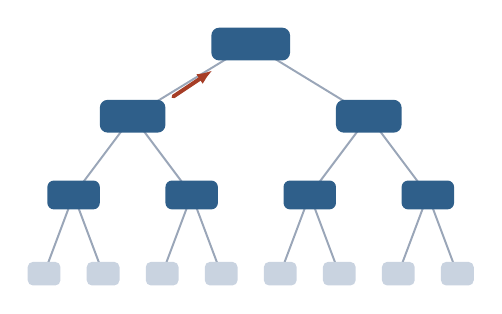
\begin{tikzpicture}[pxgrid]
  \begin{scope}[wire, line width=3\px]
    \draw (380,60) -- (200,170) (380,60) -- (560,170);
    \draw (200,170) -- (110,290) (200,170) -- (290,290) (560,170) -- (470,290) (560,170) -- (650,290);
    \foreach \p/\c in {110/65,110/155,290/245,290/335,470/425,470/515,650/605,650/695} \draw (\p,290) -- (\c,410);
  \end{scope}
  \fill[steel, rounded corners=12\px] (320,35) rectangle ++(120,50);
  \fill[steel, rounded corners=12\px] (150,145) rectangle ++(100,50) (510,145) rectangle ++(100,50);
  \foreach \x in {70,250,430,610} \fill[steel, rounded corners=10\px] (\x,268) rectangle ++(80,44);
  \foreach \x in {40,130,220,310,400,490,580,670} \fill[mist, rounded corners=8\px] (\x,392) rectangle ++(50,36);
  \draw[rust, line width=6\px, line cap=round, -{Latex[length=0.2cm]}] (262,140) -- (322,100);
\end{tikzpicture}
\end{column}
\begin{column}{0.50\textwidth}
\textbf{Bags} are sets of wires at tree nodes; leaves are final positions.\par\medskip
\textbf{Each stage}, every bag runs a constant-depth separator. It sends a few extreme items \textcolor{rust}{\textbf{up}} and splits the rest between its children.\par\medskip
\textbf{Capacities shrink} geometrically, so after $O(\log n)$ stages everything sits at the leaves, sorted.
\end{column}
\end{columns}
\note{The analysis tracks the strangeness of each item: how many levels it must climb to reach a bag whose interval contains its true rank. The invariant says items of high strangeness are exponentially rare. Depth equals the number of stages times the separator depth, and the separator, built from expander-based halvers, is where the huge constant comes from.}
\end{frame}

% ======================= 15. Constants =======================
\begingroup\altstyle
\begin{frame}{Comparing constants in the same units}{Outcome 2 \textperiodcentered\ Constants}
\begin{columns}[t]
\begin{column}{0.56\textwidth}
\small
\begin{tabular}{ll}
\toprule
\textbf{Construction} & $c$ in $c\cdot\log_2 n$ layers\\
\midrule
Paterson (1990) & $\approx 6{,}100$\\
Chv\'atal (1992), $n\ge 2^{78}$ & $\approx 1{,}830$\\
Seiferas, his sample parameters & $514{,}246$\\
Seiferas, corrected and optimized & $281{,}084$\\
Refined bookkeeping & $\approx 6{,}300$ (unreviewed)\\
\bottomrule
\end{tabular}\par\vspace{0.15cm}
{\scriptsize\color{muted}Seiferas's quoted 6.05 and 6.95 count stages, not layers.}
\end{column}
\begin{column}{0.40\textwidth}
\begin{card}[rust]{A missing term}One of Seiferas's constraints ignores a bag's own outsiders pushing items across the middle. A 100-item example shows the gap; his main theorem survives.\end{card}
\begin{caveat}[Open Math model results to be added]\end{caveat}
\end{column}
\end{columns}
\note{Constants in this literature are quoted in different units, which makes them hard to compare. Converting to comparator layers shows Seiferas's simplified analysis has an enormous constant. We also found that one of his three parameter constraints omits a term: with 5 small outsiders, 50 left-natives and 45 right-natives, exact sorting sends 5 left-natives to the wrong child, but his bound gives zero. Paterson's version includes the term. The specific improved constants from the Open Math model still need to be filled in here, matching the placeholder in the report.}
\end{frame}
\endgroup

% ======================= 16. Multiway merge =======================
\begingroup\altstyle
\begin{frame}{Merge many sorted lists at once}{Outcome 3 \textperiodcentered\ Shallower networks}
\begin{columns}[c]
\begin{column}{0.29\textwidth}\begin{step}{1}Split each of the $k$ sorted lists into its even- and odd-position elements.\end{step}\end{column}
\begin{column}{0.04\textwidth}\centering\rarrow\end{column}
\begin{column}{0.29\textwidth}\begin{step}{2}Merge all the evens, and in parallel all the odds, recursively.\end{step}\end{column}
\begin{column}{0.04\textwidth}\centering\rarrow\end{column}
\begin{column}{0.29\textwidth}\begin{step}{3}Interleave, then fix up with $\lceil\log_2 k\rceil$ extra layers.\end{step}\end{column}
\end{columns}
\vspace{0.4cm}
\begin{statement}
{\scriptsize\color{muted}The key saving is in the base case\par}\smallskip
{\color{navy}Drop the first layer of an optimal 16-wire sorter: what is left merges 8 sorted pairs in 8 layers, one fewer than the standard recursion.}
\end{statement}
\note{This is a k-way version of Batcher's odd-even merge, essentially Lee and Batcher's multiway merge from 1995. Merging k lists of length 2m costs the merge of k lists of length m plus ceiling of log k layers. The proof uses the zero-one principle: after interleaving, the sequence looks like zeros, then a block of alternating 01 pairs whose length is the number of lists with an odd count of zeros, then ones. Each cleanup layer halves that block. Our gain over Lee and Batcher comes from starting the recursion from an optimal 16-wire sorter.}
\end{frame}
\endgroup

% ======================= 17. Depths =======================
\begin{frame}{One layer better than known constructions at 128 and 1024}{Outcome 3 \textperiodcentered\ Results}
\begin{tabular}{p{0.11\textwidth}p{0.15\textwidth}p{0.17\textwidth}p{0.11\textwidth}p{0.26\textwidth}}
\toprule
$n$ & \textbf{Batcher} & \textbf{Lee--Batcher} & \textbf{Ours} & \textbf{Built from}\\
\midrule
\rowcolor{hl} 128 & 28 & 27 & \textbf{26} & $8\times 16$, then merge\\
256 & 36 & 34 & 34 & $2\times 128$, then merge\\
512 & 45 & 43 & 43 & $2\times 256$, then merge\\
\rowcolor{hl} 1024 & 55 & 53 & \textbf{52} & $8\times 128$, then merge\\
\bottomrule
\end{tabular}\par\vspace{0.4cm}
At 256 and 512 the networks beat Batcher but only match Lee and Batcher. No published depths beyond 64 inputs were found to compare against.
\note{Depths are number of layers. The Lee-Batcher column is our own arithmetic from their formula. The highlighted rows are the genuine improvements. At 256 we only match the Lee-Batcher value. Dobbelaere's well-known tables stop at 64 inputs, so the absence of a better published value is not proof of novelty.}
\end{frame}

% ======================= 18. Verification =======================
\begingroup\altstyle
\begin{frame}{How we know the networks sort}{Outcome 3 \textperiodcentered\ Verification}
Checking all $2^{1024}$ zero-one inputs is impossible. Instead, an independent checker reads only the list of layers, rediscovers the structure, and checks each piece on every input that piece can receive.\par\vspace{0.3cm}
\begin{columns}[t]
\begin{column}{0.31\textwidth}\begin{card}{16-wire blocks}All $2^{16}$ inputs\end{card}\end{column}
\begin{column}{0.31\textwidth}\begin{card}{Base mergers}All $3^8$ inputs of 8 sorted pairs\end{card}\end{column}
\begin{column}{0.31\textwidth}\begin{card}{Cleanup layers}Every input they can receive, by induction\end{card}\end{column}
\end{columns}
\vspace{0.3cm}
\begin{columns}[t]
\begin{column}{0.48\textwidth}\textbf{Negative controls:} 6 broken networks, each missing one comparator, were all rejected.\end{column}
\begin{column}{0.48\textwidth}\textbf{Cross-checks:} the 128-wire merger on all $7\times10^9$ sorted-block inputs, with no failures.\end{column}
\end{columns}
\note{The checker does not trust the builder: it works from the flat list of comparators. A short induction shows that passing these local checks implies the whole network sorts, using the zero-one principle. The negative controls show the checker is not vacuous. The 256 and 512 networks are two copies of a smaller certified network plus Batcher's merge, which we checked on all pairs of sorted halves.}
\end{frame}
\endgroup

% ======================= 19. Negative results =======================
\begin{frame}{What did not work, and why}{Other attempts}
\begin{columns}[t]
\begin{column}{0.31\textwidth}\begin{card}{Asymptotic lower bound}{\rmfamily\bfseries\large\color{navy}$3\log n$, not 4\par}\smallskip A short potential-function proof gives Yao's 2.41 and then $3\log n$. It cannot beat the known 3.27.\end{card}\end{column}
\begin{column}{0.31\textwidth}\begin{card}{Removing the tree}{\rmfamily\bfseries\large\color{navy}Sliding windows fail\par}\smallskip A fixed schedule of local halvers fails to sort for large $n$, whatever the wiring.\end{card}\end{column}
\begin{column}{0.31\textwidth}\begin{card}{Simple potentials}{\rmfamily\bfseries\large\color{navy}Distance is not enough\par}\smallskip Shrinking total displacement by a constant factor needs $\Omega(\log n)$ layers, so proofs need something like AKS's tree.\end{card}\end{column}
\end{columns}
\vspace{0.3cm}
{\color{navy}Every $O(\log n)$ network must keep long comparators until the end: after the first $\log_2 n-1$ layers, the remaining layers still need total span $n/2$.}
\note{These negative results explain why AKS looks the way it does. Long comparators are needed until the very end, which is why AKS keeps sending items back to the root. A potential based only on how far items are from home cannot contract quickly, so any proof needs an extra term playing the role of tree level and strangeness. The attempt to replace the tree with sliding windows was refuted for every wiring.}
\end{frame}

% ======================= 20. Errors =======================
\begingroup\altstyle
\begin{frame}{Errors the agents made, caught on review}{Lessons}
\begin{columns}[t]
\begin{column}{0.54\textwidth}
\begin{itemize}\setlength{\itemsep}{4pt}
\item A lemma used to rebuild the $3.27\log n$ bound was false (4-wire counterexample).
\item A proof skipped the step where values change wires.
\item A claimed $D(12)\ge 8$ came from a search bug.
\item A search pruning rule was unsound.
\item A ``$6\log n+12$'' depth came from a weak adversary.
\item A ``new'' reduction was folklore.
\end{itemize}
\end{column}
\begin{column}{0.42\textwidth}
\begin{card}[rust]{Takeaway}Agent output reads equally confident whether right or wrong. Independent checkers, counterexample searches and negative controls caught these errors.\end{card}
\end{column}
\end{columns}
\note{A significant part of the value of this project was in the review process. Several claims looked plausible and were stated confidently, but were wrong. The ones that survived are those that passed independent re-derivation, exhaustive checks on small cases, or certificate checkers tested with deliberately broken inputs.}
\end{frame}
\endgroup

% ======================= 21. Open problems =======================
\begingroup\darkstyle
\begin{frame}{Where to go next}{Open problems}
\begin{enumerate}\setlength{\itemsep}{8pt}
\color{mist}
\item Is $D(2n)\ge D(n)+3$? The case $n=16$ alone would give $D(32)\ge 12$.
\item Can $\sqrt n$ sorted lists of length $\sqrt n$ be merged in $O(\log n)$ depth by a simple network? That would give a simple $O(\log n)$ sorter.
\item What is the correct form of the lemma behind $3.27\log n$, and can it reach $4\log n$?
\item Is there a short, complete AKS proof with an explicit, reasonable constant?
\end{enumerate}
\note{These are the sharpest questions the project left open. The second is particularly attractive: merging square-root-n lists of length square-root-n in logarithmic depth would immediately give a simple logarithmic-depth sorting network by recursion. Small concrete targets are merging 4 lists of 4 in depth 6 and 8 lists of 8 in depth 13; the current best for the latter is 14.}
\end{frame}
\endgroup

\end{document}
